\documentclass{standalone}
\usepackage{tikz}


\begin{document}

  \begin{tikzpicture}[xscale=1.2,yscale=1.]
  % limits
  \def\xa{ -0.2}
  \def\xb{pi+0.4}
  \def\ya{-.2}
  \def\yb{ 1.2}
  \def\N{150} % number of points
  % axes & grid
  \draw[->,thick]
    (\xa,0) -- (\xb,0)
    node[right] {$x$};
  \draw[->,thick]
    (0,\ya) -- (0,\yb)
    node[left] {$y$};
  % functions
  \draw (0,0.70710678) -- (pi,0.70710678);
  \draw (pi/4,0.70710678) -- (pi/4,0.);
  \draw (3*pi/4,0.70710678) -- (3*pi/4,0.);
  \draw[fill=blue] (pi/4,0) circle (.03cm);
  \draw[fill=blue] (3*pi/4,0) circle (.03cm);
  \draw[thick,color=blue,samples=\N,domain=\xa:\xb] % SIN
    plot(\x,{sin(\x r)}) % r for radians
    node[above right] at (pi/2-0.7,1) {$\sin(x)$};
  % ticks
  \draw[] % x \contour{white}{$\x^\circ$}};
    node[below right,scale=0.9] at (     0, 0) {0}
    node[below,scale=0.9] at (  pi/2, 0) {$\nicefrac{\pi}{2}$}
    node[below,scale=0.9] at (  pi/4, 0) {$x_1$}
    node[below,scale=0.9] at (  3*pi/4, 0) {$x_2$}
    node[below,scale=0.9] at (  pi,   0) {\contour{white}{$\pi$}};
  \draw[] % y
    node[left,scale=0.9] at ( 0, 0.70710678) {$y$};    
\end{tikzpicture}

\end{document}